\section{Goals}

\begin{frame}[t]
	\frametitle{Goals}

	\vfill
	{\fontsize{10}{6}
		Define class \texttt{GSpline} type that is capable to represent
		\begin{itemize}
			\item Solutions of the generalized  Minimum-X problem: a \emph{convex} combination of norms of derivatives
			      \begin{eqnarray*}
				      &&\min \int_{t_0}^{t_f} \alpha_1 \left\|\diff{\qv}{t}\right\|^2 + \alpha_2 \left\|\diffk{\qv}{t}{2}\right\|^2 + \cdots  + \alpha_1 \left\|\diffk{\qv}{t}{k} \right\|^2 \d t \\
				      &&\qv(t_i) = \wp_i \ \ t_i\ \text{ is unknown}
			      \end{eqnarray*}
			\item The following transformations of the trajectory
			      \begin{itemize}
				      \item Derivatives
				      \item Elementary linear operations
				      \item Linear Scaling
			      \end{itemize}
		\end{itemize}
	}
	\vfill
\end{frame}
\begin{frame}[t]
	\frametitle{Achieving Our Goal Through Variational Principles}

	We consider the problem of the minimization of a \emph{convex} combination of norms of the derivatives

	\begin{eqnarray*}
		&&\min \int_{t_0}^{t_f} \alpha_1 \left\|\diff{\qv}{t}\right\|^2 + \alpha_2 \left\|\diffk{\qv}{t}{2}\right\|^2 + \cdots  + \alpha_1 \left\|\diffk{\qv}{t}{k} \right\|^2 \d t \\
		&&\qv(t_i) = \wp_i \ \ t_i\ \text{ is unknown!}
	\end{eqnarray*}

	Thanks to the \emph{Calculus of variations} we know that any minimizer solves the Euler-Lagrange equations

	\begin{equation*}
		-\alpha_1 \diffk{\qv}{t}{2}+ \alpha_2 \diffk{\qv}{t}{4}- \cdots +  {(-1)}^k \alpha_k \diffk{\qv}{t}{2k}= 0 \ \ \text{a.e.}
	\end{equation*}

\end{frame}

\begin{frame}[t]
	\frametitle{Achieving Our Goal Through Variational Principles}
	{\fontsize{9}{5}
		We call a \texttt{GSpline} a solution of
		\begin{equation*}
			-\alpha_1 \diffk{\qv}{t}{2}+ \alpha_2 \diffk{\qv}{t}{4}- \cdots +  {(-1)}^k \alpha_k \diffk{\qv}{t}{2k}= 0 \ \ \text{a.e.}
		\end{equation*}
		Any \texttt{GSpline} Have the following properties
		\begin{itemize}
			\item Analytical Consistency
			      \begin{equation*}
				      \diffk{}{t}{k}:\text{GSpline}\longrightarrow \text{GSpline}
			      \end{equation*}
			\item Algebraic Consistency I
			      \begin{eqnarray*}
				      +:\text{GSpline}\times\text{GSpline}\longrightarrow \text{GSpline}\\
				      \cdot:\mathbb{R} \times \text{GSpline}\longrightarrow \text{GSpline}
			      \end{eqnarray*}
			\item Algebraic Consistency II
			      \begin{eqnarray*}
				      \left[t \rightarrow \sigma t \right]:\text{GSpline}\longrightarrow \text{GSpline}
			      \end{eqnarray*}
		\end{itemize}
	}
\end{frame}
\begin{frame}[t]
	\frametitle{Goals: Monoid property}
	\begin{itemize}
		\item We desire to achieve the monoid property on the derivative, scaling and addition/scalar multiplication operations. These operation will become a monoid under the composition.
		\item Composition is a fundamental tool in programming, the Monoid structure is the most fundamental compositional structure
	\end{itemize}
	\vskip 1cm
	\begin{center}
		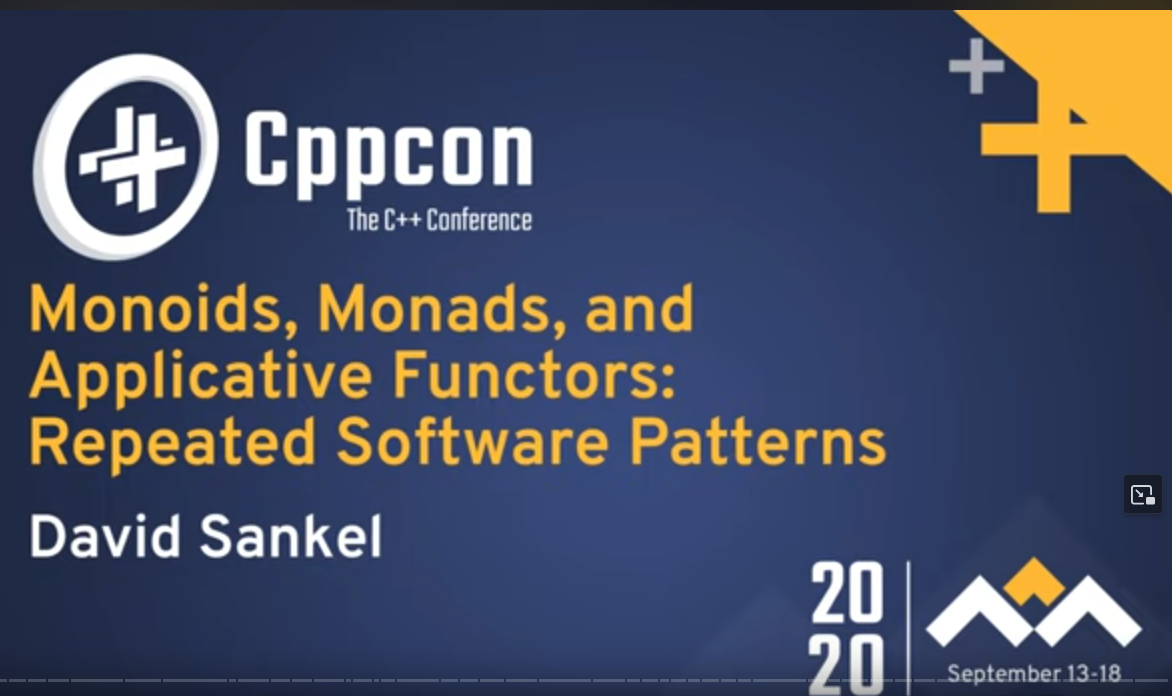
\includegraphics[height=0.2\textwidth]{./images/ccpconMonoids.png}
		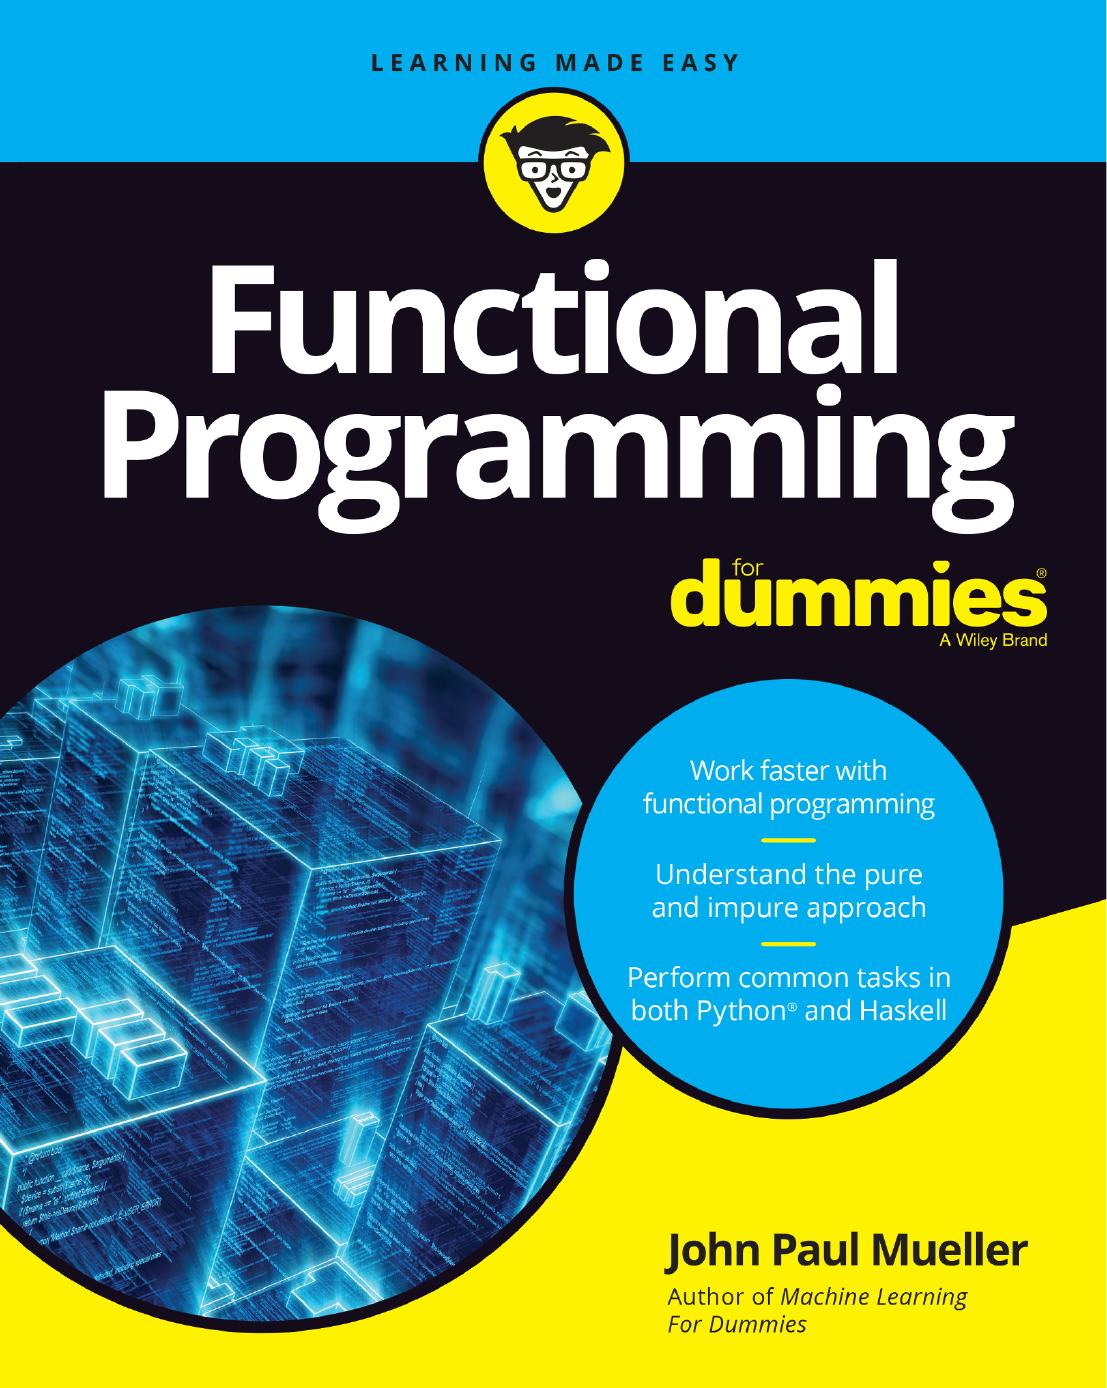
\includegraphics[height=0.2\textwidth]{./images/FunctionalProgrammingForDummies.jpeg}
		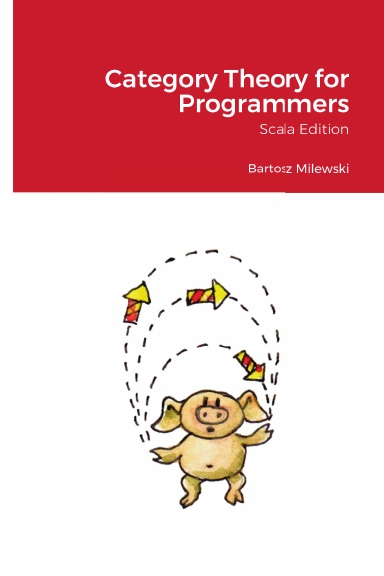
\includegraphics[height=0.2\textwidth]{./images/categoryTheoryForProgrammers.jpg}
	\end{center}
\end{frame}
